\newcommand{\ptab}{\hspace*{0.5cm}}

\newcommand{\spinlockLib}{
  $\kw{void}\ lock(l)\ \{$ \\
  \ptab $\kw{repeat}\ \{\}$ \\
  \ptab $\kw{until}\ CAS(l, 0, 1);$ \\
  $\}$ \\
  
  $\kw{void}\ unlock(l)\ \{$\\
  \ptab$\writeInst{l}{0};$\\
  $\}$
}

\newcommand{\spinlockClientII}{
  \begin{figure}[h]
    \centering
    \begin{tabular}{l || l}
      \multicolumn{2}{c}{$\writeInst{l}{0}{}$} \\
      \hline
      $lock(l);$ & $lock(l);$ \\
      $unlock(l);$ & $unlock(l);$ \\
    \end{tabular}
  \end{figure}    
}

\newcommand{\spinlockClientIIExtSep}{
  \begin{figure}[h]
    \centering
    \begin{tabular}{p{3cm} || p{3cm}}
      \multicolumn{2}{c}{$\writeInst{l_1}{0}{}; \writeInst{d_1}{0}{}; \writeInst{l_2}{0}{}; \writeInst{d_2}{0}{};$} \\
      \hline
      $lock(l_1);$ & $lock(l_2);$ \\
      $\readInst{r}{d_1};$ & $\readInst{r}{d_2};$ \\
      $\writeInst{d_1}{r + 1};$ & $\writeInst{d_2}{r + 1};$ \\
      $unlock(l_1);$ & $unlock(l_2);$ \\
    \end{tabular}
  \end{figure}    
}
\newcommand{\spinlockClientIIExt}{
  \begin{figure}[h]
    \centering
    \begin{tabular}{p{2cm} || p{2cm}}
      \multicolumn{2}{c}{$\writeInst{l}{0}{}; \writeInst{d}{0}{}$} \\
      \hline
      $lock(l);$ & $lock(l);$ \\
      $\readInst{r}{d};$ & $\readInst{r}{d};$ \\
      $\writeInst{d}{r + 1};$ & $\writeInst{d}{r + 1};$ \\
      $unlock(l);$ & $unlock(l);$ \\
    \end{tabular}
  \end{figure}    
}

% \newcommand{\spinlockClientPC}{
%   \begin{figure}[h]
%     \centering
%     \begin{tabular}{l || l}
%       \multicolumn{2}{c}{$\writeInst{l}{0}{}; \writeInst{d}{0}{}$} \\
%       \hline
%       $lock(l);$ & $lock(l);$ \\
%       $\writeInst{d}{1};$ & $\readInst{r}{d}\comment{1};$ \\
%       $unlock(l);$ & $unlock(l);$ \\
%     \end{tabular}
%   \end{figure}    
% }
\newcommand{\messagePassing}{
  \begin{figure}[h]
    \centering
    \begin{tabular}{l || l}
      \multicolumn{2}{c}{$\writeInst{f}{0}{}; \writeInst{d}{0}{}$} \\
      \hline
      $\writeInst{d}{1};$ & $\kw{while} (!\ \readInst{r}{f})\ \{\};$ \\
      $\writeInst{f}{1};$ & $\readInst{r}{d}\comment{1};$ \\
    \end{tabular}
  \end{figure}    
}


\newcommand{\spinlockClientMany}{
  \begin{figure}[h]
    \centering
    \begin{tabular}{l || l || l}
      \multicolumn{3}{c}{$\writeInst{l}{0}{}$} \\
      \hline
      $lock();$ & {$\ldots$} & $lock();$ \\
      % {} & {$\ldots$} & {} \\
      $unlock();$ & {}  & $unlock();$ \\
    \end{tabular}
  \end{figure}
}

\newcommand{\spinlockLibClientII}{
  \begin{minipage}[c]{0.25\linewidth}
    \spinlockLib
  \end{minipage}
  \begin{minipage}[c]{0.25\linewidth}
    \spinlockClientII
  \end{minipage}
}
\newcommand{\spinlockLibClientIIVert}{
  \begin{minipage}[c]{0.25\linewidth}
    \spinlockLib
    \vspace{-0.5cm}
    \spinlockClientII
  \end{minipage}
}


\newcounter{evctr}
\newcommand{\curEv}{\theevctr}
\newenvironment{traceenv}[2]
{
  \setcounter{evctr}{0}
  \begin{tikzpicture}[xscale=#1, yscale=#2]
}
{
  \node (T1) at (-0.5 * 1, 1) {\textbf{Thread 1}};
  \node (T2) at (-0.5 * 1, 0) {\textbf{Thread 2}};
  \node (E1) at (0, 0.5) {}; \node (E2) at (\curEv, 0.5) {};
  % \dpo{E1}{E2};
  \draw[time] (E1) edge node[] { } (E2);
  \node (timePic) at (\curEv + 0.25, 0.5) {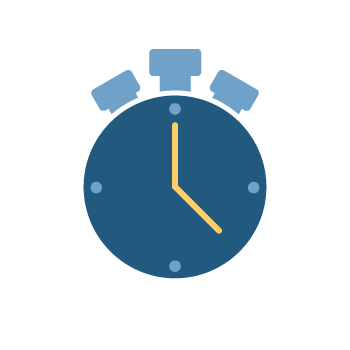
\includegraphics[width=0.1\textwidth]{time.png}};
  \end{tikzpicture}
}

\newcommand{\SCDeclUnfair}{
  \begin{figure}[h]
    \centering
    \begin{tabular}{p{3cm} || p{3cm}}
      \multicolumn{2}{c}{$\writeInst{x}{0}{}$} \\
      \hline
      $\writeInst{x}{1};$ & $\kw{while} (\kw{true})\ \{$ \\
      $\kw{while} (\kw{true})\ \{$ & $\quad \writeInst{x}{2};$ \\
      $\quad \readInst{r}{x};\comment{1,1,\ldots}$ & $\}$ \\
      $\}$ & ${}$ \\
    \end{tabular}
  \end{figure}
}

\newcommand{\SCDeclUnfairEvents}{
  \node (W1) at (0 * \hof, -0 * \vof) {$\evlab{\lW}{}{x}{1}$};
  \node (R11) at (0 * \hof, -1 * \vof) {$\evlab{\lR}{}{x}{1}$};
  \node (R12) at (0 * \hof, -2 * \vof) {$\evlab{\lR}{}{x}{1}$};
  \node (R1inf) at (0 * \hof, -2.5 * \vof) {$\ldots$};

  \node (W21) at (1 * \hof, -0 * \vof) {$\evlab{\lW}{}{x}{2}$};
  \node (W22) at (1 * \hof, -1 * \vof) {$\evlab{\lW}{}{x}{2}$};
  \node (W2inf) at (1 * \hof, -1.5 * \vof) {$\ldots$};
    
  % \dpo{L1}{R1}; \dpo{R1}{W1}; \dpo{W1}{U1}; 
  % \dpo{L2}{R2}; \dpo{R2}{W2}; \dpo{W2}{U2};         
}


\newcommand{\spinlockInfGraphEvents}{      
      \node (U1) at (0 * \hof, -0 * \vof) {$\evlab{\lU}{}{l}{0, 1}$};
      \node (W1) at (0 * \hof, -2 * \vof) {$\evlab{\lW}{}{l}{0}$};

      \node (R21) at (1 * \hof, -0 * \vof) {$\evlab{\lR}{}{l}{1}$};
      \node (R22) at (1 * \hof, -2 * \vof) {$\evlab{\lR}{}{l}{1}$};
      \node (R23) at (1 * \hof, -4 * \vof) {$\evlab{\lR}{}{l}{1}$};
      \node (R24) at (1 * \hof, -5 * \vof) {$\ldots$};
}
\newcommand{\spinlockInfGraphPO}{
      \dpo{U1}{W1};
      \dpo{R21}{R22}; \dpo{R22}{R23};
}
\newcommand{\spinlockInfGraphRF}{
      \node (W0) at (0.5 * \hof, 1 * \vof) {$\evlab{\lW}{}{l}{0}$};
      \drf{W0}{U1};
      \drf{W1}{R21}; \drf{W1}{R22}; \drf{W1}{R23};
}
\newcommand{\spinlockInfGraphMO}{    
      \dmo[bend left=30]{W0}{U1}; \dmo[bend right=30]{U1}{W1};
}
\newcommand{\spinlockInfGraphComments}{
      \node (V1) at (0.5, -4) {}; \node (V2) at (1.5, -4) {};
      \draw[po] (V1) edge node[yshift=0.2cm, right] { } (V2);
      \node at (1, -4.5) {``program order''};      
}

\newcommand{\spinlockFinGraphEvents}{
      % \node (W0) at (0.5 * \hof, 1 * \vof) {$\evlab{\lW}{}{l}{0}$};
      
      \node (U1) at (0 * \hof, -0 * \vof) {$\evlab{\lU}{}{l}{0, 1}$};
      \node (W1) at (0 * \hof, -2 * \vof) {$\evlab{\lW}{}{l}{0}$};

      \node (R21) at (2 * \hof, -0 * \vof) {$\evlab{\lR}{}{l}{1}$};
      \node (R22) at (2 * \hof, -2 * \vof) {$\evlab{\lR}{}{l}{1}$};
      \node (U2) at (2 * \hof, -4 * \vof) {{\color{green} $\evlab{\lU}{}{l}{0, 1}$}};
      \node (W2) at (2 * \hof, -6 * \vof) {$\evlab{\lW}{}{l}{0}$};
}
\newcommand{\spinlockFinGraphRelations}{
      \dpo{U1}{W1};
      \dpo{R21}{R22}; \dpo{R22}{U2}; \dpo{U2}{W2};

      % \drf{W0}{U1};
      % \drf{W1}{R21}; \drf{W1}{R22};
      \drf{W1}{U2};

      % \dmo[bend left=30]{W0}{U1}; \dmo[bend right=30]{U1}{W1};
}

    

%%% Local Variables:
%%% mode: latex
%%% TeX-master: "oopsla"
%%% End:
